\documentclass[conference]{IEEEtran}
\IEEEoverridecommandlockouts
\usepackage{setspace}
\usepackage{gensymb}
\singlespacing
\usepackage[cmex10]{amsmath}
\usepackage{amsthm}
\usepackage{mathrsfs}
\usepackage{txfonts}
\usepackage{stfloats}
\usepackage{bm}
\usepackage{cite}
\usepackage{cases}
\usepackage{subfig}
\usepackage{longtable}
\usepackage{multirow}
\usepackage{enumitem}
\usepackage{mathtools}
\usepackage{tikz}
\usepackage{circuitikz}
\usepackage{verbatim}
\usepackage[breaklinks=true]{hyperref}
\usepackage{tkz-euclide} % loads  TikZ and tkz-base
\usepackage{listings}
\usepackage{color}    
\usepackage{array}    
\usepackage{longtable}
\usepackage{calc}     
\usepackage{multirow} 
\usepackage{hhline}   
\usepackage{ifthen}   
\usepackage{lscape}     
\usepackage{chngcntr}
\usepackage{algorithm}
\usepackage[indLines=false]{algpseudocodex}
\DeclareMathOperator*{\Res}{Res}
\renewcommand\thesection{\arabic{section}}

\renewcommand\thesubsection{\thesection.\arabic{subsection}}
\renewcommand\thesubsubsection{\thesubsection.\arabic{subsubsection}}

\renewcommand\thesectiondis{\arabic{section}}
\renewcommand\thesubsectiondis{\thesectiondis.\arabic{subsection}}
\renewcommand\thesubsubsectiondis{\thesubsectiondis.\arabic{subsubsection}}
\renewcommand\thetable{\arabic{table}}
% correct bad hyphenation here
\hyphenation{op-tical net-works semi-conduc-tor}
\def\inputGnumericTable{}                                 %%

\renewcommand\algorithmicensure{\textbf{Input:}}
\newcommand{\algorithmautorefname}{Algorithm}
\renewcommand{\sectionautorefname}{Section}

\lstset{
%language=C,
frame=single, 
breaklines=true,
columns=fullflexible,
literate=
{-}{$\rightarrow{}$}{1},
}
%\lstset{
%language=tex,
%frame=single, 
%breaklines=true
%}

\DeclareMathOperator*{\argmax}{arg\,max}
\DeclareMathOperator*{\argmin}{arg\,min}
\begin{document}
\newtheorem{theorem}{Theorem}[section]
\newtheorem{problem}{Problem}
\newtheorem{proposition}{Proposition}[section]
\newtheorem{lemma}{Lemma}[section]
\newtheorem{corollary}[theorem]{Corollary}
\newtheorem{example}{Example}[section]
\newtheorem{definition}[problem]{Definition}
\newcommand{\BEQA}{\begin{eqnarray}}
\newcommand{\EEQA}{\end{eqnarray}}
\newcommand{\define}{\stackrel{\triangle}{=}}
\providecommand{\mbf}{\mathbf}
\providecommand{\pr}[1]{\ensuremath{\Pr\left(#1\right)}}
\providecommand{\qfunc}[1]{\ensuremath{Q\left(#1\right)}}
\providecommand{\sbrak}[1]{\ensuremath{{}\left[#1\right]}}
\providecommand{\lsbrak}[1]{\ensuremath{{}\left[#1\right.}}
\providecommand{\rsbrak}[1]{\ensuremath{{}\left.#1\right]}}
\providecommand{\brak}[1]{\ensuremath{\left(#1\right)}}
\providecommand{\lbrak}[1]{\ensuremath{\left(#1\right.}}
\providecommand{\rbrak}[1]{\ensuremath{\left.#1\right)}}
\providecommand{\cbrak}[1]{\ensuremath{\left\{#1\right\}}}
\providecommand{\lcbrak}[1]{\ensuremath{\left\{#1\right.}}
\providecommand{\rcbrak}[1]{\ensuremath{\left.#1\right\}}}
\theoremstyle{remark}
\newtheorem{rem}{Remark}
\newcommand{\sgn}{\mathop{\mathrm{sgn}}}
\providecommand{\abs}[1]{\left\vert#1\right\vert}
\providecommand{\res}[1]{\Res\displaylimits_{#1}} 
\providecommand{\norm}[1]{\left\lVert#1\right\rVert}
\providecommand{\mtx}[1]{\mathbf{#1}}
\providecommand{\mean}[1]{E\left[ #1 \right]}   
\providecommand{\fourier}{\overset{\mathcal{F}}{ \rightleftharpoons}}
\providecommand{\system}[1]{\overset{\mathcal{#1}}{ \longleftrightarrow}}
\newcommand{\solution}{\noindent \textbf{Solution: }}
\newcommand{\cosec}{\,\text{cosec}\,}
\providecommand{\dec}[2]{\ensuremath{\overset{#1}{\underset{#2}{\gtrless}}}}
\newcommand{\myvec}[1]{\ensuremath{\begin{pmatrix}#1\end{pmatrix}}}
\newcommand{\mydet}[1]{\ensuremath{\begin{vmatrix}#1\end{vmatrix}}}
\renewcommand{\vec}[1]{\boldsymbol{\mathbf{#1}}}
\def\putbox#1#2#3{\makebox[0in][l]{\makebox[#1][l]{}\raisebox{\baselineskip}[0in][0in]{\raisebox{#2}[0in][0in]{#3}}}}
     \def\rightbox#1{\makebox[0in][r]{#1}}
     \def\centbox#1{\makebox[0in]{#1}}
     \def\topbox#1{\raisebox{-\baselineskip}[0in][0in]{#1}}
     \def\midbox#1{\raisebox{-0.5\baselineskip}[0in][0in]{#1}}

\title{SwarmBots : Autonomous Multi‑Agent Task Execution with Centralized Ultrasonic Mapping}

\author{
    \IEEEauthorblockN {B. Sumanth, Sowmith and G.V.V. Sharma} 
    %\IEEEauthorblockN{B. Sumanth} 
    %\IEEEauthorblockA{EE Department, Indian Institute of Technology Hyderabad,\\
    %\and
    %\IEEEauthorblockN{Sowmith} 
    %\and
    %\IEEEauthorblockN{G. V. V. Sharma} 
    %\and
    \IEEEauthorblockA{Department of Electrical Engineering, 
	    \\
	    Indian Institute of Technology Hyderabad,\\
    Kandi, India 502284
\\
gadepall@ee.iith.ac.in}
}

\maketitle

\begin{abstract}
  This paper presents a novel centralized framework for mapping and multi-task execution using multiple unmanned ground vehicles (UGVs). The system leverages ultrasonic sensors for environmental mapping, followed by autonomous task execution using a master-slave architecture. A user-interactive graphical interface allows manual selection of task points on the generated map. The master UGV maps the environment and broadcasts task locations to slave UGVs for autonomous execution. Experimental results demonstrate reliable mapping accuracy and robust coordination among UGVs in a controlled indoor environment.
\end{abstract}

\section{Introduction}
\label{sec:intro}
The evolution of robotics has enabled autonomous systems across logistics, agriculture, and surveillance through collaborative multi-agent behavior~\cite{brambilla2013swarm}. Most commercial solutions, however, rely on costly technologies like LiDAR, GPS, and high-performance processors, making them unsuitable for small-scale indoor deployments~\cite{kalra2005hoplite}.
%\subsection*{1.1 Problem Statement}

Multi-robot coordination has been extensively studied, with emphasis on areas like SLAM, dynamic task allocation, and swarm behavior~\cite{brambilla2013swarm, kalra2005hoplite}.  A deep reinforcement learning model (DDQN) combined with ant colony optimization for dynamic task assignment in UGV swarms was introduced in~\cite{jin2024multi}. Similarly, hierarchical approaches for UAV-UGV cooperation using global and local planners have been explored in~\cite{mdpi2022hierarchical}.

Thus, there is a lack of low-cost, modular systems that can perform indoor multi-UGV mapping and task execution without relying on infrastructure-dependent technologies. Current methods are either too expensive, too centralized, or lack user-friendly interfaces for real-time coordination in constrained environments.

%, gadepalli2023future}.

In this paper, a cost-efficient architecture is employed by integrating time-aware task distribution, ESP-NOW communication, and manual path annotation. 
This is done by proposing a centralized control system using ESP32 microcontrollers, ultrasonic sensors~\cite{arduino_hcsr04}, and ESP-NOW communication~\cite{espnowguide}. An intuitive web-based GUI built with SPIFFS~\cite{randomnerd2024esp32} allows users to assign tasks and direct swarm behavior interactively, without external routing hardware. Our framework supports scalable swarm control for research and prototyping~\cite{jin2024multi, mdpi2022hierarchical}
%, gadepalli2023future}.
%, though it is possible to use affordable sensors (like HC-SR04) in tandem with ESP-based embedded systems to create real-time indoor mapping systems with GUI-driven task delegation~\cite{arduino_hcsr04, espnowguide, randomnerd2024esp32}

\section{Proposed Navigation System}
\label{sec:proposed-system}

The proposed architecture for multi-UGV coordination is detailed in this section. Each UGV contains hardware for communication and autonomous navigation. With a central master UGV, the system can autonomously execute tasks. Key components of the system include
\begin{enumerate}
	\item {\em Collaborative Mapping Using Ultrasonic Sensors:}
Ultrasonic modules (HC-SR04) mounted on the master UGV scan surroundings using a grid traversal strategy. Position is estimated via RPM-based dead reckoning, and obstacle data is processed into a 2D occupancy grid map~\cite{arduino_hcsr04}
%, gadepalli2023future}.
The complete environment map is constructed in real-time and visualized via the GUI.
%
\item {\em Dead Reckoning for Localization: }
Each UGV computes its position based on wheel rotations (RPM), using:
\begin{equation}
\text{Distance} = \frac{\text{RPM} \times \pi \times \text{Diameter} \times \Delta t}{60}
\end{equation}
This allows real-time navigation feedback without relying on GPS or encoders.

\item {\em Time-Aware Task Distribution Algorithm:}
After the user assigns points via the GUI, the master UGV estimates travel time to each target. Tasks are segmented and distributed proportionally to each slave’s expected duration to maximize parallelism and reduce idle time~\cite{jin2024multi}.

\item {\em Peer-to-Peer Communication with ESP-NOW:}
ESP32 modules communicate using ESP-NOW—a low-latency, MAC-based protocol. It eliminates the need for a Wi-Fi router, offering robustness for offline, indoor multi-agent systems~\cite{espnowguide}.

\item {\em GUI-Based Human Interaction Layer:}
The GUI is hosted on the master UGV and serves as the primary human-machine interface~\cite{randomnerd2024esp32}. It enables the following functionalities:
\begin{itemize}
    \item Canvas-based path drawing Users can draw custom paths or regions directly onto the grid map for task planning.
    \item Click-based task selection Individual grid points can be selected to assign discrete tasks to UGVs.
    \item Real-time feedback of UGV positions Each UGV's estimated location is updated and visualized on the interface.
    \item Task status visualization Task execution states (e.g., pending, in-progress, completed) are reflected dynamically on the GUI.
\end{itemize}
%
\item {\em Embedded Software Architecture:}
Each UGV runs modular firmware developed using either the ESP-IDF or Arduino framework, depending on complexity. The software architecture is divided into:
\begin{itemize}
    \item \textbf{Master UGV:} Responsible for path segmentation, task scheduling, and GUI synchronization. It acts as a bridge between the user and slave units.
    \item \textbf{Slave UGVs:} Execute motion control routines, update position through RPM-based dead reckoning, and report task status back to the master.
\end{itemize}
\end{enumerate}

Firmware modules are structured to separate communication, control logic, sensor interfacing, and utility functions for maintainability and reusability. The platform is engineered for deployment in resource-constrained environments, enabling scalable swarm behaviors through compact embedded logic and lightweight communication protocols.

\begin{figure}[t]
    \centering
    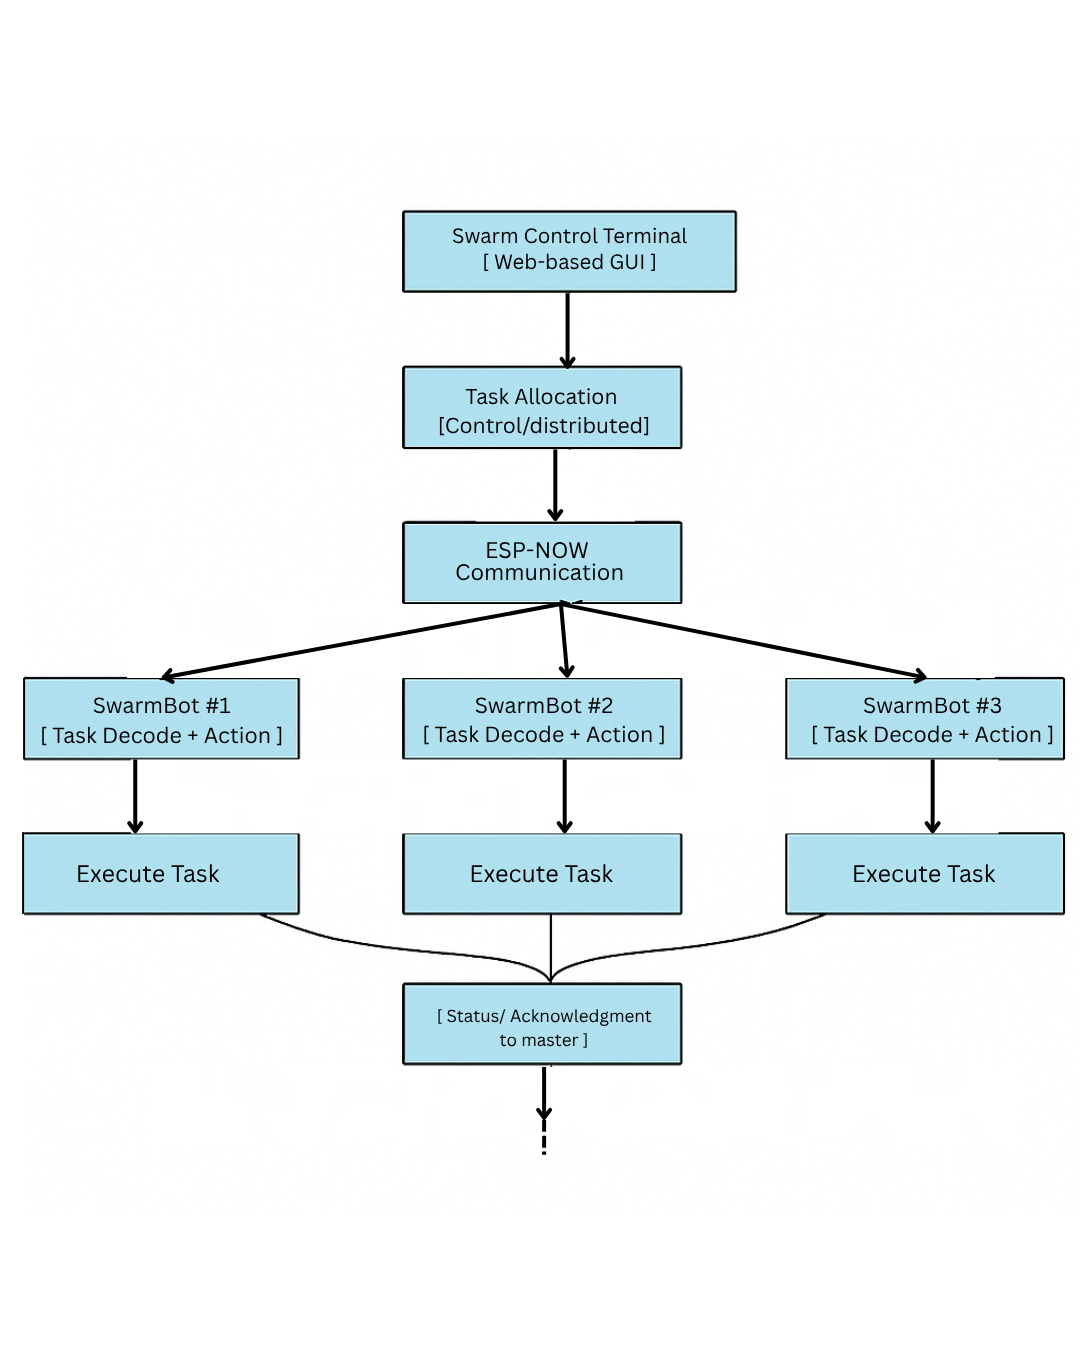
\includegraphics[width=\columnwidth]{figs/Swarm Block.png}
  \caption{SwarmBots system architecture: GUI-driven task allocation, ESP‑NOW communication, autonomous execution, and status feedback.}
  \label{fig:system-architecture}
\end{figure}

\section{Methodology}
\label{sec:Methodology}

\subsection{Mapping Phase}
The master UGV performs 2D environmental mapping by traversing the environment in a structured grid pattern. It uses ultrasonic distance sensors~\cite{arduino_hcsr04} to gather obstacle data, which is fused with positional estimates obtained via dead reckoning~\cite{kalra2005hoplite}. A 2D occupancy grid is constructed dynamically to represent free and occupied spaces in the environment.

\subsection{GUI-Based Task Assignment}
The real-time occupancy grid is rendered on the GUI, allowing users to visually inspect the environment and select target task points. These click-based inputs are encoded into coordinate values and transmitted wirelessly to the master UGV for further processing~\cite{espnowguide}.

\subsection{Task Distribution Strategy}
Once the master UGV receives the task coordinates, it allocates them to the slave UGVs based on either \cite{}:

\begin{itemize}
    \item Round-robin assignment: Tasks are distributed sequentially to each available slave UGV.
    \item Distance-based allocation: Each task is assigned to the nearest available slave UGV, minimizing traversal time.
\end{itemize}

This strategy ensures balanced workload distribution and reduces the likelihood of navigation conflicts or congestion~\cite{jin2024multi}.

\subsection{Execution Phase}
Upon receiving their assigned task coordinates, slave UGVs begin autonomous navigation. Navigation is achieved through time-based motor control \cite{} or simple PID algorithms \cite{}.
%~\cite{gadepalli2023future}. 
On reaching the target, each UGV performs the associated operation, such as flashing an LED, taking sensor readings, or signaling task completion to the master.


\section{Implementation}
\label{sec:Implementation}

The complete source code and setup for the SwarmBots system are available on 
\begin{center}
  \url{https://github.com/gadepall/SWARMBOTS}
\end{center}

\subsection{Assets}
\begin{enumerate}
    \item UGV chassis with DC motors
    \item ESP32 microcontroller with Type-B USB cable
    \item L293D Motor Driver IC
    \item Breadboard and Jumper Wires
    \item Ultrasonic Sensor (HC-SR04)
    \item Android Phone or Laptop for GUI (optional if GUI is pre-hosted)
    \item (Optional) USB 2.0/3.0 Hub
\end{enumerate}
\subsection{Procedure}
\begin{enumerate}
    \item Build the UGVs using ESP32, motor driver, and ultrasonic sensors as per the wiring diagram provided in the repo.
    \item Connect each ESP32 to your Android phone or laptop via USB.
    \item For firmware compilation, open terminal and run:
        \begin{lstlisting}
$ cd SWARMBOTS/master_firmware
$ pio run
        \end{lstlisting}
    \item Upload firmware using ArduinoDroid (for Android users) or PlatformIO (on PC):
        \begin{lstlisting}
Actions - Upload - Upload Precompiled
        \end{lstlisting}
    and choose the firmware file at
        \begin{lstlisting}
codes/.pio/build/firmware.hex
        \end{lstlisting}
   
\item 
Repeat for slave bots:
        \begin{lstlisting}
$ cd SWARMBOTS/slave_firmware
$ pio run
        \end{lstlisting}
        \item Access the GUI:

Open browser and navigate to the ESP32-hosted web server.

Draw or click on task points in the occupancy map.

The master UGV will distribute tasks accordingly.


         \item  Power on the UGVs in an open indoor environment. The master starts mapping; slaves receive task commands and execute them autonomously.
          \item  Monitor real-time updates and robot positions via the GUI interface. 
          
\end{enumerate}
\section{Results}
\label{sec:results}
The SwarmBots system was tested in a structured indoor environment using a master-slave configuration of three UGVs. The key outcomes of the experiment are summarized below

Reliable Mapping Accuracy: The master UGV successfully generated a real-time 2D occupancy map using only ultrasonic data and dead reckoning. Spatial features such as walls and obstacles were distinguishable without requiring GPS, LIDAR, or encoders.

\subsection{Interactive GUI Performance} 
The GUI enabled smooth human-robot interaction. Users could assign target points via simple clicks, and receive 
real-time visual feedback on robot positions and task progress.

\subsection{Autonomous Multi-UGV Task Execution}
Slave UGVs performed assigned tasks in parallel with high independence. Each UGV navigated to its target using internal logic, and task completion was communicated back to the master without human intervention.

\subsection{Position Estimation Precision}
Experimental trials demonstrated a positional accuracy within ±5 cm, sufficient for typical indoor navigation and task execution scenarios.

\subsection{System Scalability}
The framework scaled effectively with multiple UGVs. Task distribution strategies (round-robin and distance-based) helped avoid collisions and ensured balanced workloads.

\subsection{Low-Cost, High-Impact}
All experiments were conducted using off-the-shelf ESP32 boards and basic sensors, underscoring the potential of this architecture in resource-constrained deployments.

\section{Conclusion and Future Work}
\label{sec:conclusion}
In this work, we developed and demonstrated a low-cost, modular, and scalable system for autonomous task execution using a swarm of Unmanned Ground Vehicles (UGVs). Our approach integrated ultrasonic-based mapping, RPM-based dead reckoning, and a user-friendly GUI for task coordination. The system successfully enabled collaborative mapping and parallel task execution in an indoor setting without relying on GPS, LiDAR, or expensive sensors.
The experiments confirmed the reliability of position estimation, real-time feedback, and decentralized task handling using ESP-NOW communication. The architecture proved to be robust, scalable, and efficient for indoor robotic coordination, even with hardware constraints and future work includes.

\begin{itemize}
\item Incorporating IMU and optical encoders to enhance localization accuracy
\item Implementing advanced obstacle avoidance using IR or vision-based sensors
\item Developing adaptive task reassignment algorithms based on real-time status
\item Extending the system to semi-structured outdoor environments with longer range communication
\item Introducing swarm-level intelligence to support dynamic decision-making and reconfiguration
\end{itemize}

\bibliographystyle{IEEEtran}
\bibliography{references}

\end{document}
